\documentclass[a4paper,11pt]{article}
\usepackage[big]{layaureo}
\usepackage{amsmath,amssymb}
\usepackage[default,regular,bold]{sourceserifpro}
\usepackage[regular,semibold]{sourcesanspro}
\usepackage[T1]{fontenc}
\usepackage[utf8]{inputenc}
\usepackage{textcomp} % provide euro and other symbols
\usepackage[]{microtype}
\usepackage{xcolor}
\usepackage{longtable,booktabs,array}
\usepackage{calc} % for calculating minipage widths
\usepackage{pdfpages}
\usepackage{graphicx}
\usepackage{sectsty}
\usepackage{setspace}
\usepackage[hidelinks]{hyperref}
\usepackage{hyperxmp}
\usepackage[
    type={CC},
    modifier={zero},
    version={1.0},
]{doclicense}
\usepackage{outlines}

\hypersetup{
pdftitle={Cash or Card? Game Design Document},
pdfauthor={Andrea Franceschini},
pdfcreationdate={2023-10-09},
pdfmoddate={2023-10-09},
pdfversionid={1.0},
pdflang={en-GB},
pdfsubject={{Game Design Document}},
}

\title{%
	Cash or Card?\\
	\large{Game Design Document}}
\author{Andrea Franceschini}
\date{1 July 2023}

\onehalfspacing

\makeatletter
\renewcommand{\maketitle}{\bgroup\setlength{\parindent}{0pt}
\begin{flushleft}
	\sffamily\LARGE\@title
\end{flushleft}\egroup
}
\makeatother

\begin{document}

% \setstretch{1.25}

\maketitle

\noindent Help a shopkeeper get paid: customers prefer paying cash or card and you
will decide whether to accept it or propose an alternative! Accept cash
to feel it rustle between your fingers or embrace the convenience of
electronic payments? The choice is yours! But be careful because every
choice has consequences. Insurance premium or banking fees? Risk of
robbery or losing a customer? Choose your strategy, see the consequences
and explore the advantages, disadvantages and reasons behind each
choice!
\\

\noindent\textbf{Genre}: Puzzle, simulation

\section{High level concept}\label{high-level-concept}

\subsection{Target audience}\label{target-audience}

General population. The aim is to educate the players about the costs,
risks, and opportunities associated with different payment methods.

\begin{itemize}
\item
  Adults (18+) are the primary target audience as they are more likely
  to regularly handle payments and have a payment card or other
  electronic payment method.
\item
  Young adults (13-18) are somewhat likely to handle payments, although
  they are unlikely to use non-cash payment methods. Young adults are an
  important target audience as they are soon going to turn into the
  primary audience, therefore it is important that they get early
  exposure to the content.
\item
  Children (8-13) are secondary as target audience, although important
  in the long run, and as influencer of their parents and guardians. In
  financial matters, children tend to get exposed second-hand to choices
  made by their parents and guardians, and often take these choices
  acritically. It is important for them to be exposed to the different
  sides of the debate so that they can feel confident in asking
  questions and discussing it with adults.
\end{itemize}

\subsection{Unique selling points}\label{unique-selling-points}

There are more customers than shopkeepers. The shopkeepers tend to have
very strong views and a very defensive attitude towards their preferred
payment choices. It is not easy for customers to understand and discuss
the shopkeepers' perspective -- i.e., trust me, you don't know what it's
like to run a shop! -- and so playing the role can be informative for
customers.

\section{Product design}\label{product-design}

\subsection{Player experience and game
POV}\label{player-experience-and-game-pov}

The player is a shopkeeper who must earn enough money to pay a big
invoice within the next 5 days.

\subsection{Visual and Audio style}\label{visual-and-audio-style}

Retro-style pixel art visuals. Chiptune-adjacent music and SFX.

\subsection{Game World}\label{game-world}

The game is played entirely inside the shopkeeper's shop with narrative
implying events (bank runs, street robberies) happening outside. The
game opens with a phone call from one of the shopkeeper's suppliers
reminding the shopkeeper they need to pay a big invoice by the end of
the week. The shopkeeper states they have still 5 days to earn the
remaining money. The game loop starts from there until the end of the
game.

\subsection{Platforms, technology,
scope}\label{platforms-technology-scope}

The game will be playable on desktop computers and mobile phones. Godot
4 is the engine.

\section{Detailed and Game Systems
Design}\label{detailed-and-game-systems-design}

\subsection{Core loop}\label{core-loop}

The game loop runs 5 times (days) as follows.

\begin{enumerate}
\def\labelenumi{\arabic{enumi}.}
\item
  Customer (NPC) approaches the check-out desk with an amount to pay and
  a payment preference (cash or card).
\item
  The player decides whether to take the payment offer or propose an
  alternative method.
\item
  The player accepts.

  \begin{enumerate}
  \def\labelenumii{\arabic{enumii}.}
  \item
    If the customer prefers card, the player is presented with three
    choices or payment methods with different payment fees. The fee is
    deducted from the total. The bank and electronic costs amounts are
    updated accordingly.
  \item
    If the customer prefers cash, the full amount is added to the cash
    amount.
  \end{enumerate}
\item
  The player rejects.

  \begin{enumerate}
  \def\labelenumii{\arabic{enumii}.}
  \item
    A dialogue starts between the customer and the player with each
    party presenting a series of common objections to using the other
    payment method.
  \item
    The player can at any point give in to the customer's request, or
    insist in the hope of changing the customer's mind.
  \item
    If the customer leaves the goods and exits the shop without paying,
    the full amount is recorded as lost income.
  \item
    If the customer or the player decide to accept a payment method, the
    payment is handled like in step 3 using the payment method agreed so
    far.
  \end{enumerate}
\item
  If there are still customers, the loop starts back from step 1.
\item
  If there are no more customers, the end of day scenario plays out.

  \begin{enumerate}
  \def\labelenumii{\arabic{enumii}.} 
  \item
    If there is cash in the till, the player must decide whether to
    leave it there until the next day (back to step 1), or take it to
    the bank.
  \item
    If the player does a bank run, unless they run into a street
    robbery, a cash deposit fee is deducted from the cash amount and is
    added to the cash costs, and the remaining amount is added to the
    bank total. This represents that cash is not as \emph{gratis} as it
    may appear. The loop starts back from step 1.
  \item
    If the player runs into a street robbery, based on the robbery
    chance, they have a choice of losing all the cash or making an
    insurance claim. If they make an insurance claim, they are refunded
    the cash amount minus the excess and the cash deposit fee, and the
    bank and cash costs are updated as in step 6.2. The insurance
    premium and excess increase. The loop starts back from step 1.
  \end{enumerate}
\end{enumerate}

At any point during a game loop (day) a shop robbery can happen based on
the robbery chance. A shop robbery is handled like in step 6.3 with the
additional cost of losing any remaining customers for the day.

\subsection{Objectives and
Progression}\label{objectives-and-progression}

The player's objective is to earn enough money at the end of 5 days to
pay a large invoice plus the insurance premium. The player's actions are
guided by the dialogues presented during the game loop.

\subsection{Game Systems}\label{game-systems}

In the first instance, the basic game system is entirely described by
the core loop. There is scope for power-ups and side-mechanics to make
the game more flexible and increase the player's control, freedom, and
immersion.

\subsection{Interactivity}\label{interactivity}

The main interaction system is the dialogue system. See figure \ref{fig:uisketch}.

\begin{figure}[h]
\centering
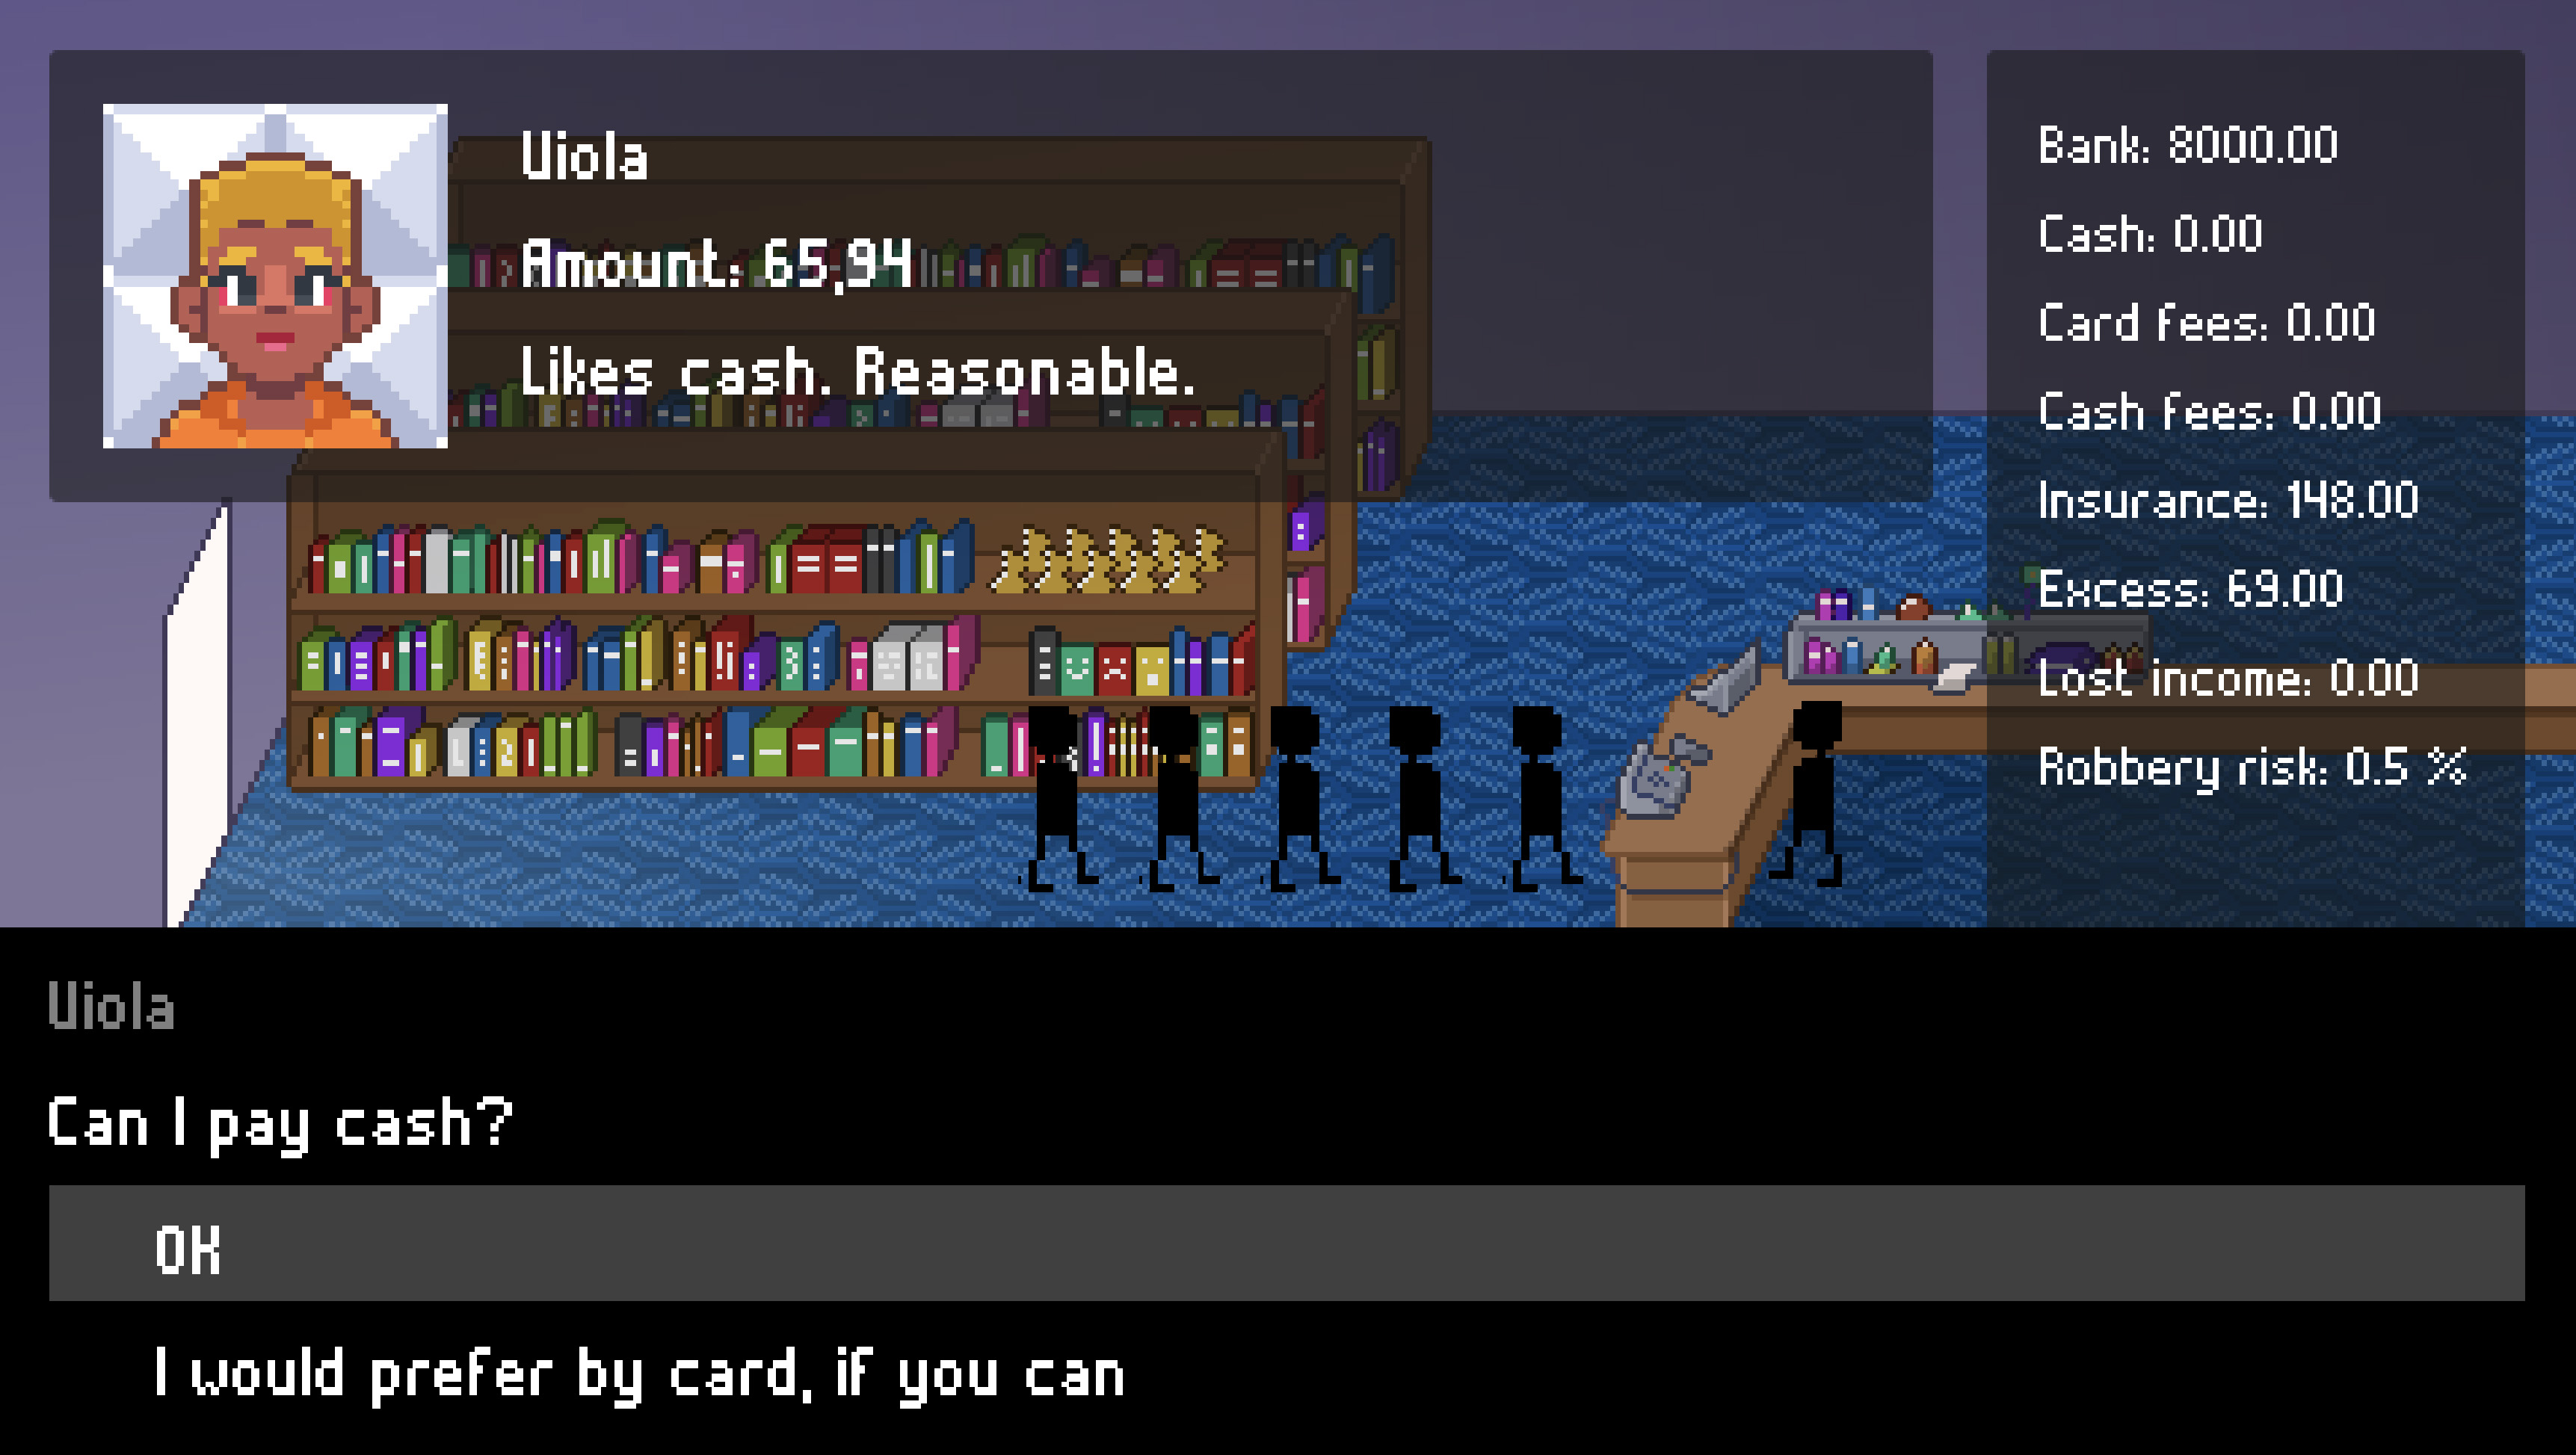
\includegraphics[width=\textwidth]{ui_sketch.jpg}
\caption{This is the caption.}\label{fig:uisketch}
\end{figure}

\end{document}
